% !TEX root =  Chapter5.tex
% !TeX spellcheck = en-GB

\subsection{Benchmarking}
Once the functionality has been confirmed to work as intended, the technique can be benchmarked to determine if there is benefit in using it for run-time efficiency. Testing was done on a personal computer with an NVIDIA GeForce MX250 Graphics Card \cite{mx250} - and while this is able to execute the CUDA code and ensure it produces the right output, it is not sufficient to gather representative benchmarking data. Using a personal computer system may result in noisy data, from the system scheduling other tasks.
\par
In order to gather better data, access to a supercomputer located in Cambridge, part of the Cambridge Service for Data-Driven Discovery (CSD3), was kindly provided - although workloads for this project were placed in a low priority queue.
\par
The supercomputer named \textit{Wilkes2} was used, which provides 4 NVidia P100 16GB Graphical Processing Units \cite{p100}. The translator currently only generates code for a single graphics card, but a possible extension would be to include MPI and divide the workload across multiple GPUs. As with many supercomputer clusters, \textit{Wilkes2} requires jobs to be submitted via SLURM \cite{slurm}.

\subsubsection{Benchmarking Strategy}
The \textit{airfoil} program is also used for benchmarking, as it is reasonably industrially representative. The input mesh remains the same as in the Testing section, with 721801 nodes, but the number of time steps is upped from 1000 to 10,000 to make any difference more noticable. OP2's internal timing funtions are used to sum the total time spent in each of the parallel loops, which can be compared between the versions with JIT compilation enabled and disabled.
\par
As seen previously in Section \ref{sss:jit_comp} (Just-in-Time Compilation), the time taken for the invocation of the compiler at run-time to complete is also recorded. It is a one-time cost at the start of execution, but still needs to be considered.
\par
Given more time other OP2 applications would also have been used to compare data, however, finding a suitable HPC system and gaining access took a larger portion of the project's duration than expected.

\subsubsection{Results}
The graph in Figure \ref{fig:res} shows the total run-time of both versions, divided sections corresponding to the total wall clock time spent in each of the parallel loops.

\begin{figure}[h!]
\begin{center}
\caption{run-time Divided by Parallel Loop}
\label{fig:res}
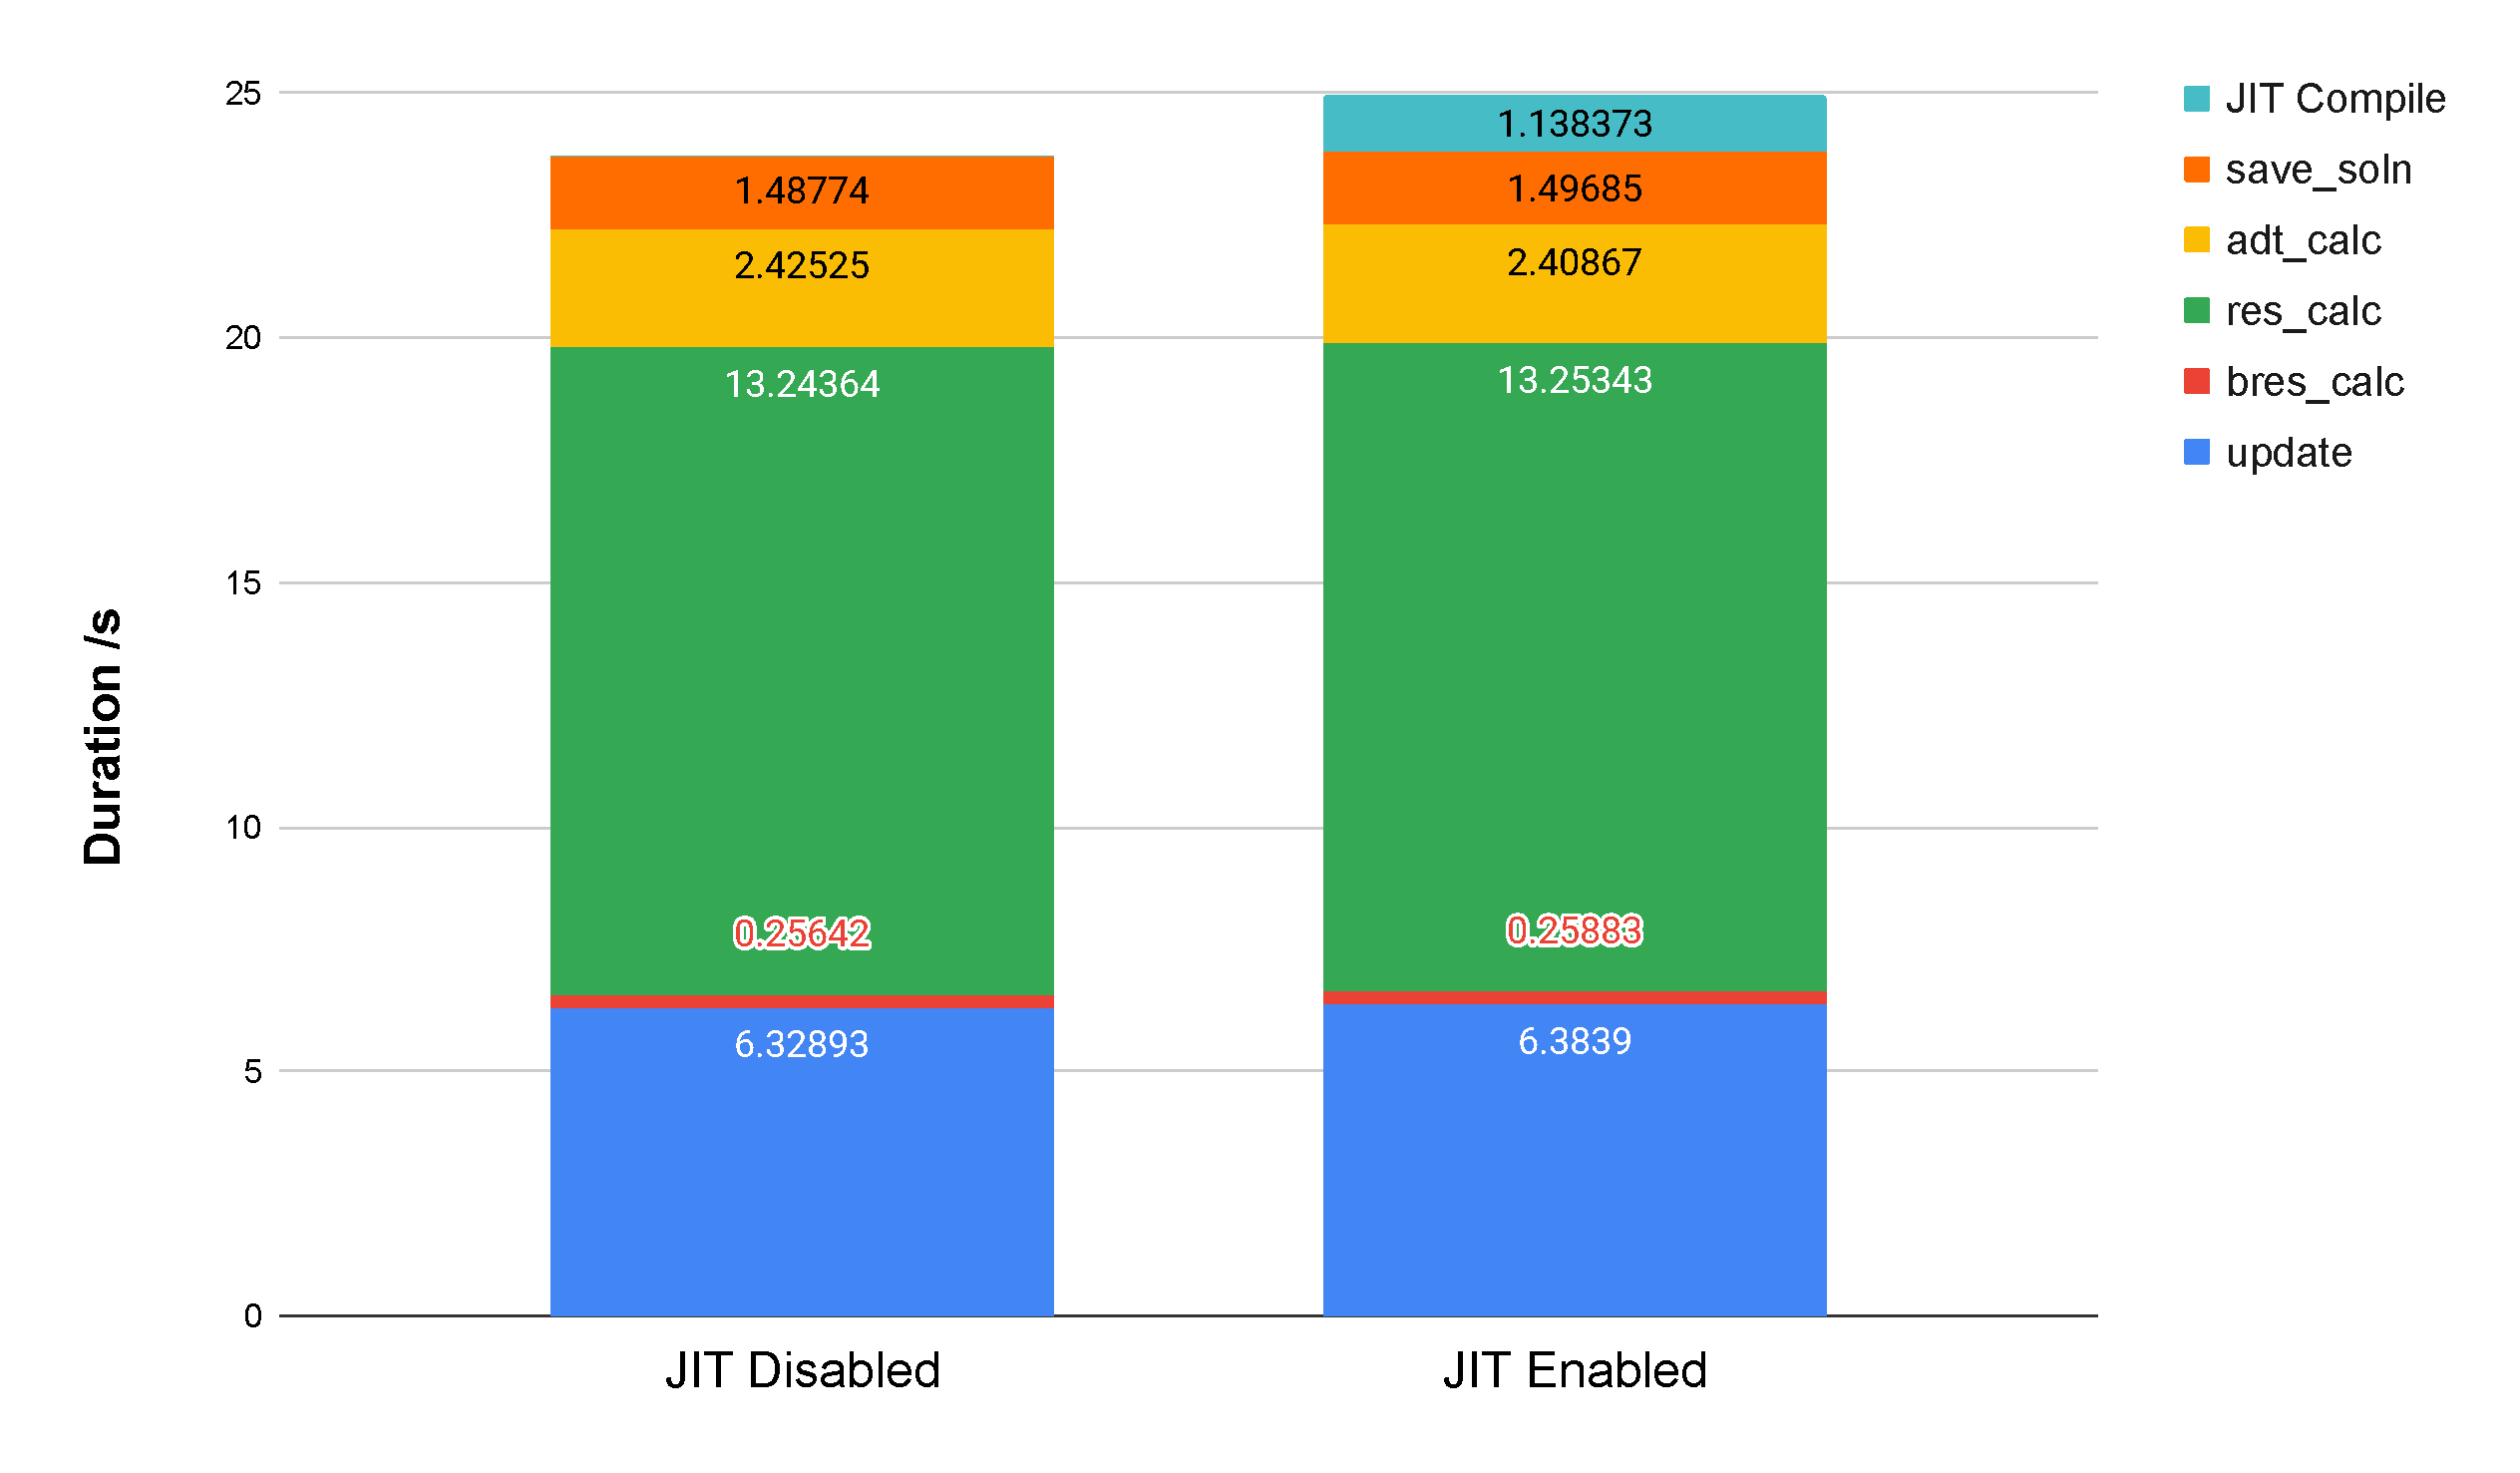
\includegraphics[width=\textwidth]{results.pdf}
\end{center}
\vspace{-1cm}
\end{figure}

\noindent Values are taken across an average of 10 executions of the binary, to further eliminate any possible noise in the JIT compilation duration.

\subsubsection{Analysis}
What Figure \ref{fig:res} clearly shows, is that the run-time has not been reduced by using the technique, and indeed is almost the same but with the addition of the time taken to invoke the compiler.
\par
It is important when drawing conclusions from this to remember that there are other assertions that can be made at run-time. Since the only assertion being made is that values declared constant will not change, the time available for optimisation is only the time taken to read constant values from memory, which will not be a significant proportion of the run-time for most projects, since CUDA-capable graphics cards have a designated section of device memory for caching constants \cite[p73]{guide}.
\par
It is true that the constants no longer need to be copied into the device memory, however this was previously only done once at the start of the program.
\par
What the results demonstrate is that more sophisticated optimisations which make use of the inputs being known need to be implemented. Since the JIT Compilation process has now been implemented, this system can continue to be used and improved upon to provide a run-time reduction to the execution of the binary. Even a small improvement to a very large solver, which might run millions of time-step iterations, could quickly re-coup and indeed begin to outweigh the relatively tiny one-time cost of recompilation.
